\documentclass[11pt]{article}
\usepackage[margin=0.72in]{geometry}
\usepackage[T1]{fontenc}
\usepackage[utf8]{inputenc}
\usepackage{lmodern}
\usepackage{microtype}
\usepackage{amsmath}
\usepackage{graphicx}
\usepackage{booktabs}
\usepackage{tabularx}
\usepackage{array}
\usepackage{longtable}
\usepackage{xcolor}
\usepackage{hyperref}
\usepackage{fancyhdr}
\usepackage{caption}
\usepackage{enumitem}
\usepackage{float}

\definecolor{ReportBlue}{HTML}{356CAD}
\definecolor{ReportTeal}{HTML}{2F9E8F}
\definecolor{ReportOrange}{HTML}{D9773D}
\definecolor{ReportGray}{HTML}{555B63}
\hypersetup{colorlinks=true,linkcolor=ReportBlue,urlcolor=ReportBlue,citecolor=ReportBlue}
\graphicspath{{Figures/}}
\setlength{\parindent}{0pt}
\setlength{\parskip}{0.55em}
\setlist[itemize]{leftmargin=1.4em,itemsep=0.25em,topsep=0.3em}
\captionsetup{font=small,labelfont=bf}
\pagestyle{fancy}
\fancyhf{}
\fancyhead[L]{EMIC/IWYMIC Performance Signal Analysis}
\fancyhead[R]{Data Through 2026}
\fancyfoot[C]{\thepage}
\renewcommand{\headrulewidth}{0.4pt}
\setlength{\headheight}{14pt}
\newcommand{\keyresult}[1]{\par\noindent\colorbox{ReportBlue!9}{\parbox{0.96\linewidth}{#1}}\par}
\newcolumntype{Y}{>{\raggedright\arraybackslash}X}

\begin{document}

\hypersetup{pageanchor=false}
\begin{titlepage}
\centering
\vspace*{1.2in}
{\color{ReportBlue}\rule{\textwidth}{1.5pt}}\\[0.55in]
{\Huge\bfseries EMIC and IWYMIC Performance as a Signal for Later Olympiad Success\par}
\vspace{0.35in}
{\Large APMO and IMO Outcomes Through 2026\par}
\vspace{0.65in}
{\large Full Statistical Analysis Report\par}
\vfill
\begin{tabular}{rl}
Fixed identity roster: & 3,112 contestants \\
EMIC/IWYMIC study years: & 2013 to 2023, excluding 2020 \\
Higher-contest endpoint: & 2026 \\
Generated: & 2026-07-23 \\
\end{tabular}
\vfill
{\color{ReportBlue}\rule{\textwidth}{1.5pt}}
\end{titlepage}

\hypersetup{pageanchor=true}
\pagenumbering{roman}
\tableofcontents
\clearpage
\pagenumbering{arabic}

\section{Executive Summary}

This report asks whether stronger performance at a contestant's first observed EMIC or IWYMIC award appearance predicts later APMO or IMO success. The analysis finds a consistent predictive association among named EMIC/IWYMIC award recipients. It does not estimate a causal effect of participation.

\keyresult{\textbf{Main result.} Adding baseline percentile to a country, contest-stage, and baseline-year model improves out-of-time average precision for all four outcomes. The improvement is 0.088 for APMO awards and 0.075 for IMO awards. Both country-cluster bootstrap intervals remain above zero.}

\begin{itemize}
\item In unrestricted follow-up through 2026, the APMO award rate rises from 4.4\% in the 25-50\% baseline band to 17.7\% in the 75-100\% band. The IMO rate rises from 5.8\% to 17.6\%.
\item At five years, the right-censored award incidence for the 75-100\% band is 16.6\% for APMO and 17.2\% for IMO. The corresponding 25-50\% rates are 4.9\% and 5.6\%.
\item Baseline award tier matters most clearly at IWYMIC. Within five years, 30.8\% of IWYMIC Gold recipients earn an APMO award and 36.6\% earn an IMO award.
\item Country remains important. Rates differ sharply across delegations, and many country intervals are wide. Performance is informative, but selection systems and training environments also shape outcomes.
\end{itemize}

\section{Data Scope and 2026 Update}

The identity universe is fixed by EMIC and IWYMIC. APMO and IMO records can enrich an existing identity but cannot add a new person. This design keeps the research question centered on former EMIC/IWYMIC contestants.

\begin{table}[H]
\centering
\caption{Contest Coverage in the Fixed Roster}
\begin{tabular}{lrrl}
\toprule
Contest & Roster Identities & Matched Appearances & Coverage \\
\midrule
EMIC & 1,814 & 2,008 & 2013 to 2023, excluding 2020 \\
IWYMIC & 1,646 & 1,900 & 2013 to 2023, excluding 2020 \\
APMO & 360 & 634 & 2016 to 2026 \\
IMO & 375 & 742 & 2013 to 2026 \\
\bottomrule
\end{tabular}
\end{table}

The official 2026 APMO report contains 397 contestants, of whom 55 match the fixed roster. The official 2026 IMO page contains 666 contestants, of whom 55 match the roster. All IMO official ranks reconcile with recomputed global score ties. All APMO award labels reconcile with the official cutoffs and country award limits.

\textbf{APMO source status.} The APMO 2026 score-level report is complete but the official site still labels it preliminary. The report is included because the user requested the current 2026 data. Its status is retained in the audit and changelog. A future refresh should be run after the official preliminary notice is removed.

\textbf{APMO source anomaly.} The APMO 2026 Vietnam rank-2 row displays problem scores totaling 18 and an official total of 25. The official total is retained for rank and award calculations. This is the only 2026 problem-total mismatch.

Official sources: \url{https://www.apmo-official.org/year_report/2026} and \url{https://www.imo-official.org/results/individual/year/2026/}.

\section{Definitions and Methods}

\subsection{Baseline and Outcomes}
\begin{itemize}
\item The unit of analysis is one reviewed contestant identity.
\item Baseline is the earliest EMIC or IWYMIC award appearance. EMIC breaks a same-year tie.
\item Baseline rank uses the average position of the full score tie. Percentile is $1 - \text{rank average}/\text{participants}$.
\item A later award is Gold, Silver, Bronze, or Honourable Mention. A later medal is Gold, Silver, or Bronze.
\item APMO and IMO outcomes must occur in a strictly later calendar year. Same-year and earlier results are excluded.
\item The primary prediction window is five calendar years. Complete-window eligibility requires all five years to be observable through 2026.
\end{itemize}

The complete five-year samples contain 1,754 contestants for APMO and 2,486 for IMO. APMO baselines before 2015 are excluded from complete-window analysis because complete contestant-level APMO data begin in 2016.

\subsection{Analytical Components}
\begin{enumerate}
\item Descriptive progression rates compare fixed baseline-percentile bands.
\item Raw quintiles and adjusted curves assess the continuous performance signal.
\item Outcome transitions connect baseline award tier to later result class.
\item Kaplan-Meier-style cumulative incidence handles right-censoring.
\item Country estimates use Wilson 95\% intervals.
\item Ridge-logistic models use forward baseline-year validation. Each test year is predicted only from earlier baseline years.
\item The baseline model uses country, stage, and baseline year. The performance model adds percentile, percentile squared, and a percentile-by-stage interaction.
\item Metric-difference intervals use 300 country-cluster bootstrap replicates with a fixed seed.
\end{enumerate}

\section{Observed Progression by Baseline Performance}

The unrestricted descriptive rates include every later record observed through 2026. They show the full observed progression but give older cohorts more follow-up time than recent cohorts.

\begin{table}[H]
\centering
\caption{Unrestricted Progression Through 2026}
\small
\begin{tabular}{lrrrrr}
\toprule
Baseline Band & Contestants & APMO Award & APMO Medal & IMO Award & IMO Medal \\
\midrule
25-50\% & 936 & 4.4\% & 2.9\% & 5.8\% & 3.8\% \\
50-75\% & 1,136 & 9.4\% & 6.4\% & 10.0\% & 6.9\% \\
75-100\% & 1,040 & 17.7\% & 14.1\% & 17.6\% & 14.9\% \\
\bottomrule
\end{tabular}
\end{table}

The top band has about 4.0 times the APMO award rate and 3.1 times the IMO award rate of the 25-50\% band. These ratios are descriptive. The fixed-window models below provide the stronger predictive test.

\begin{figure}[H]
\centering
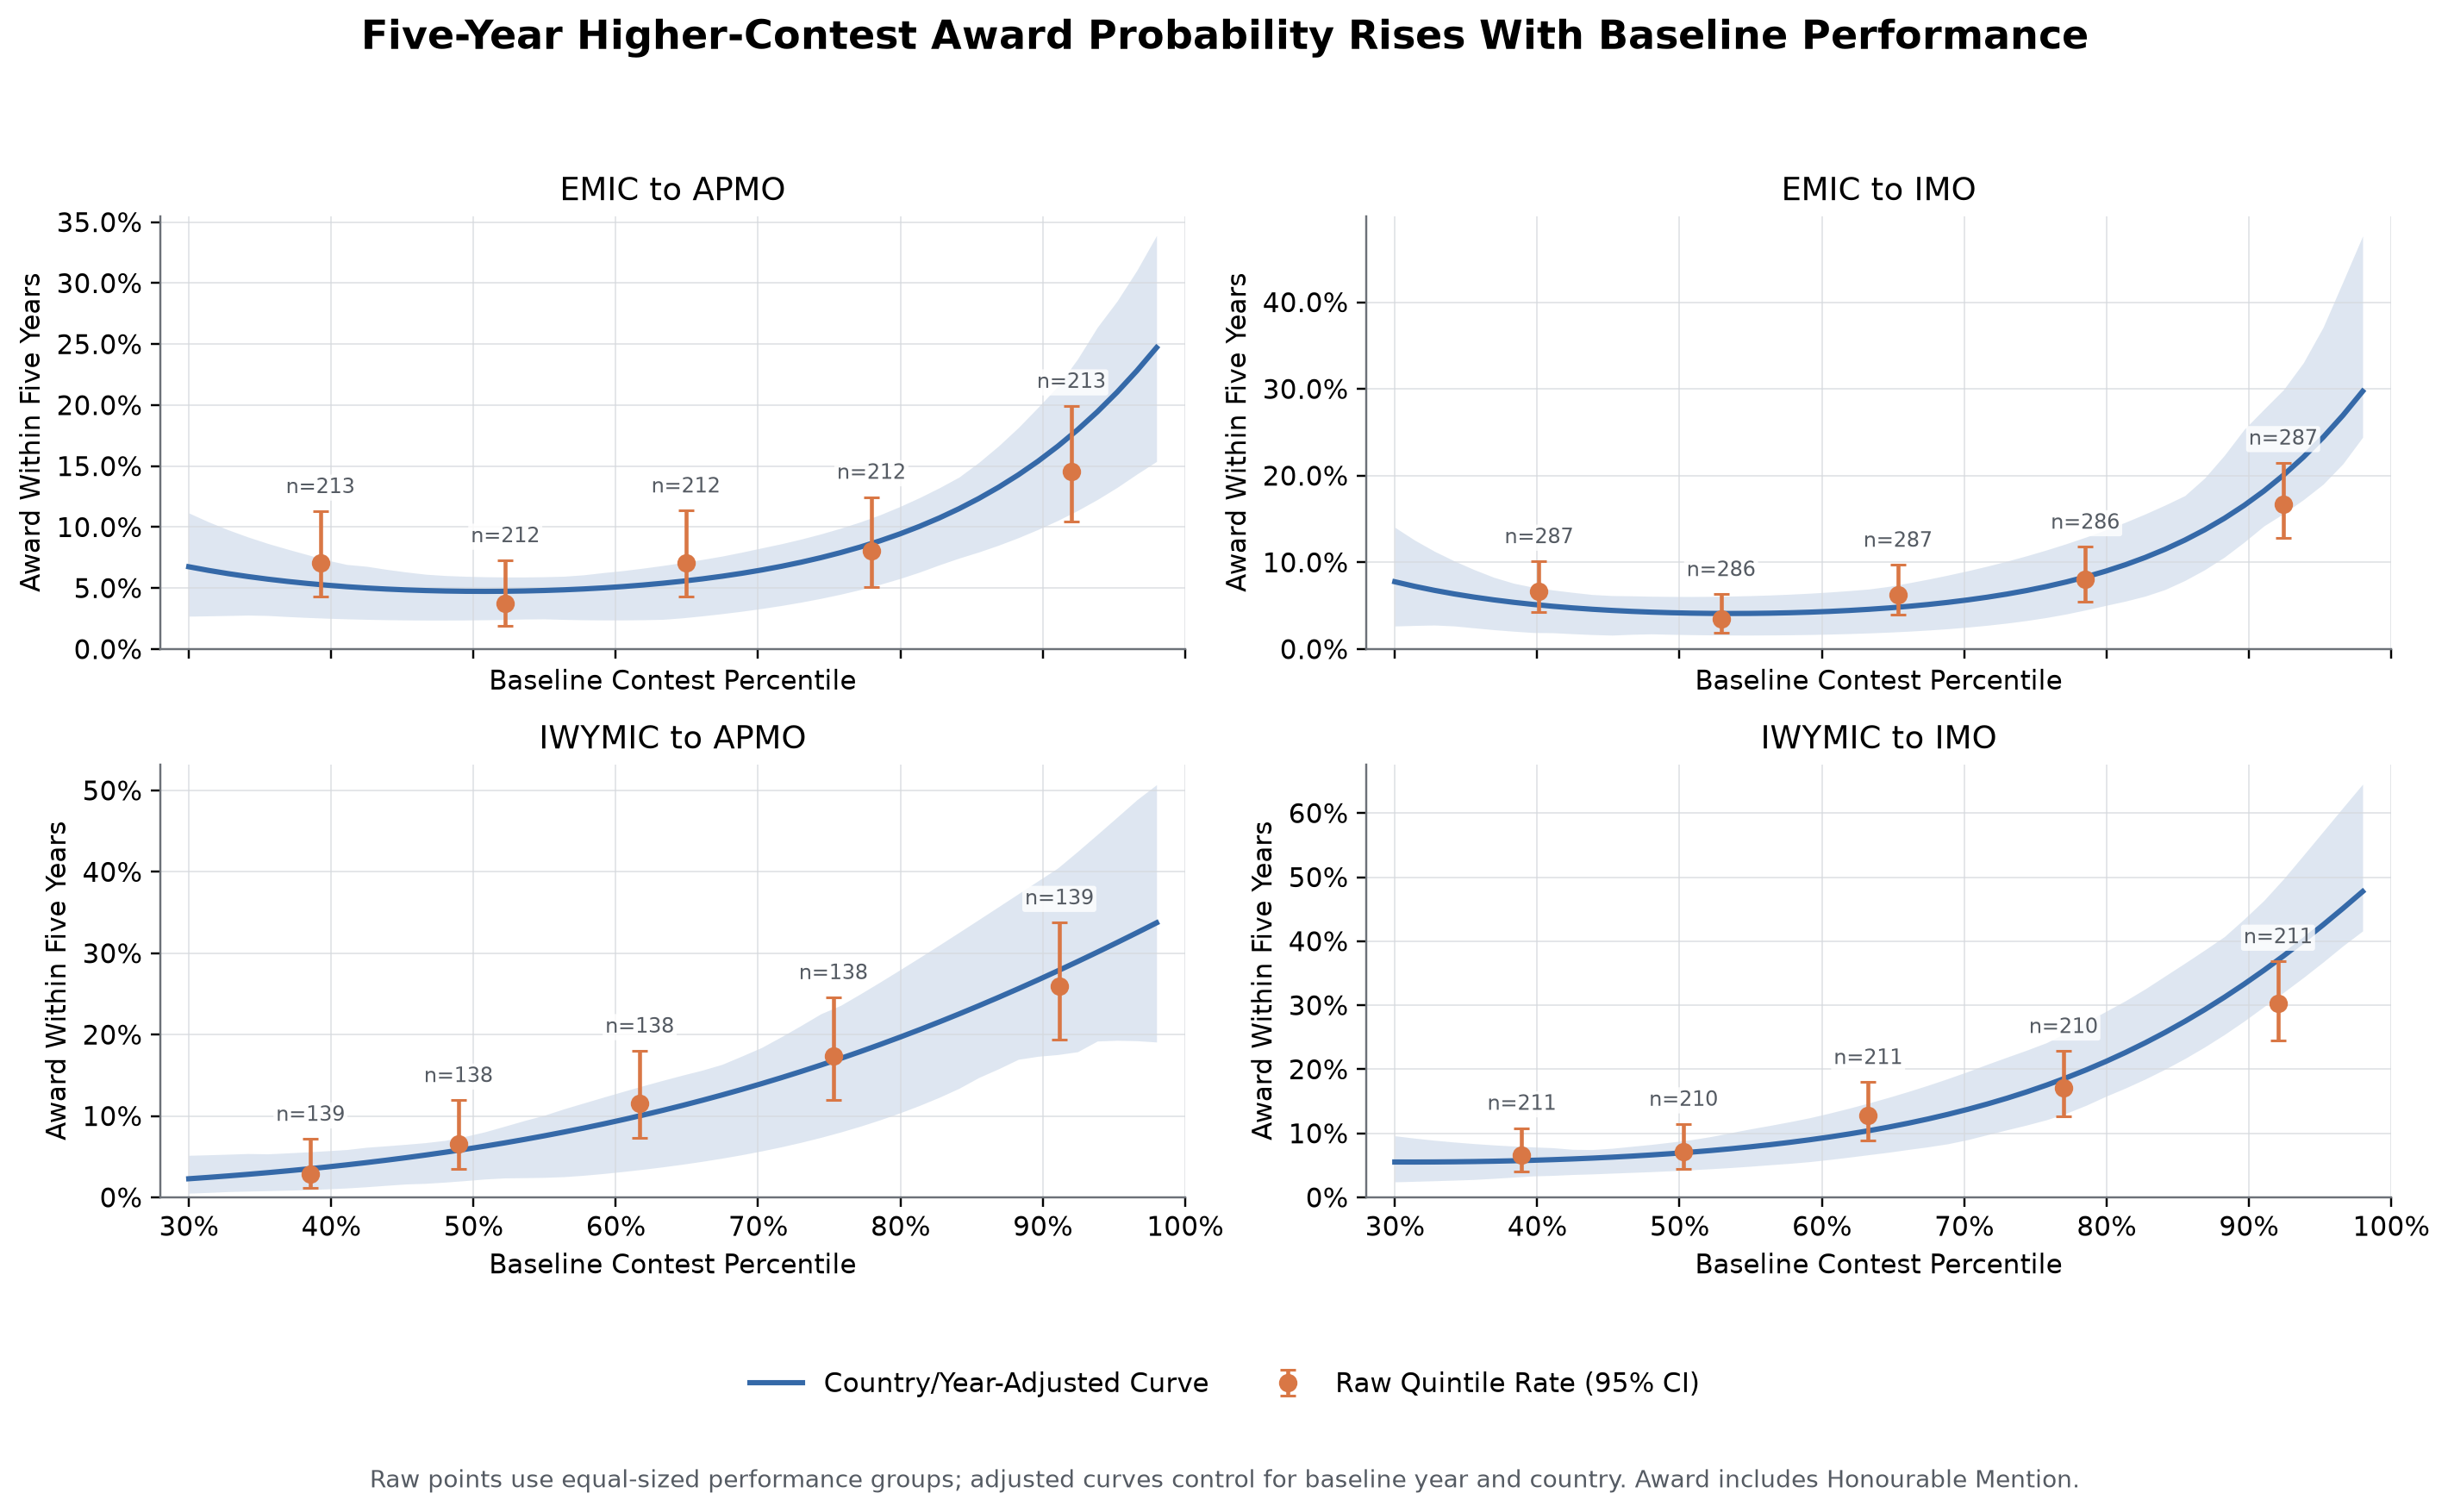
\includegraphics[width=\textwidth]{01 Performance Signal Curves.png}
\caption{Raw five-year quintile rates and country/year-adjusted curves. Labels show quintile sample sizes.}
\end{figure}

The adjusted curves rise most sharply near the upper end of the observed percentile range. IWYMIC performance has the steepest relationship with both APMO and IMO outcomes. The uncertainty bands widen near the extremes because fewer observations support those curve regions.

\section{Baseline Award Tier and Later Result Class}

Baseline medal tiers provide an ordinal sensitivity check that does not depend on the precision of the total-participant denominator. Higher baseline tiers generally lead to higher five-year award rates.

\begin{table}[H]
\centering
\caption{Five-Year Higher-Contest Award Rate by Baseline Tier}
\begin{tabular}{llrr}
\toprule
Stage & Baseline Tier & APMO Award & IMO Award \\
\midrule
EMIC & Merit & 5.9\% & 5.1\% \\
EMIC & Bronze & 6.8\% & 7.0\% \\
EMIC & Silver & 10.3\% & 8.9\% \\
EMIC & Gold & 18.6\% & 24.8\% \\
IWYMIC & Merit & 4.9\% & 7.1\% \\
IWYMIC & Bronze & 15.2\% & 14.7\% \\
IWYMIC & Silver & 21.9\% & 23.2\% \\
IWYMIC & Gold & 30.8\% & 36.6\% \\
\bottomrule
\end{tabular}
\end{table}

\begin{figure}[H]
\centering
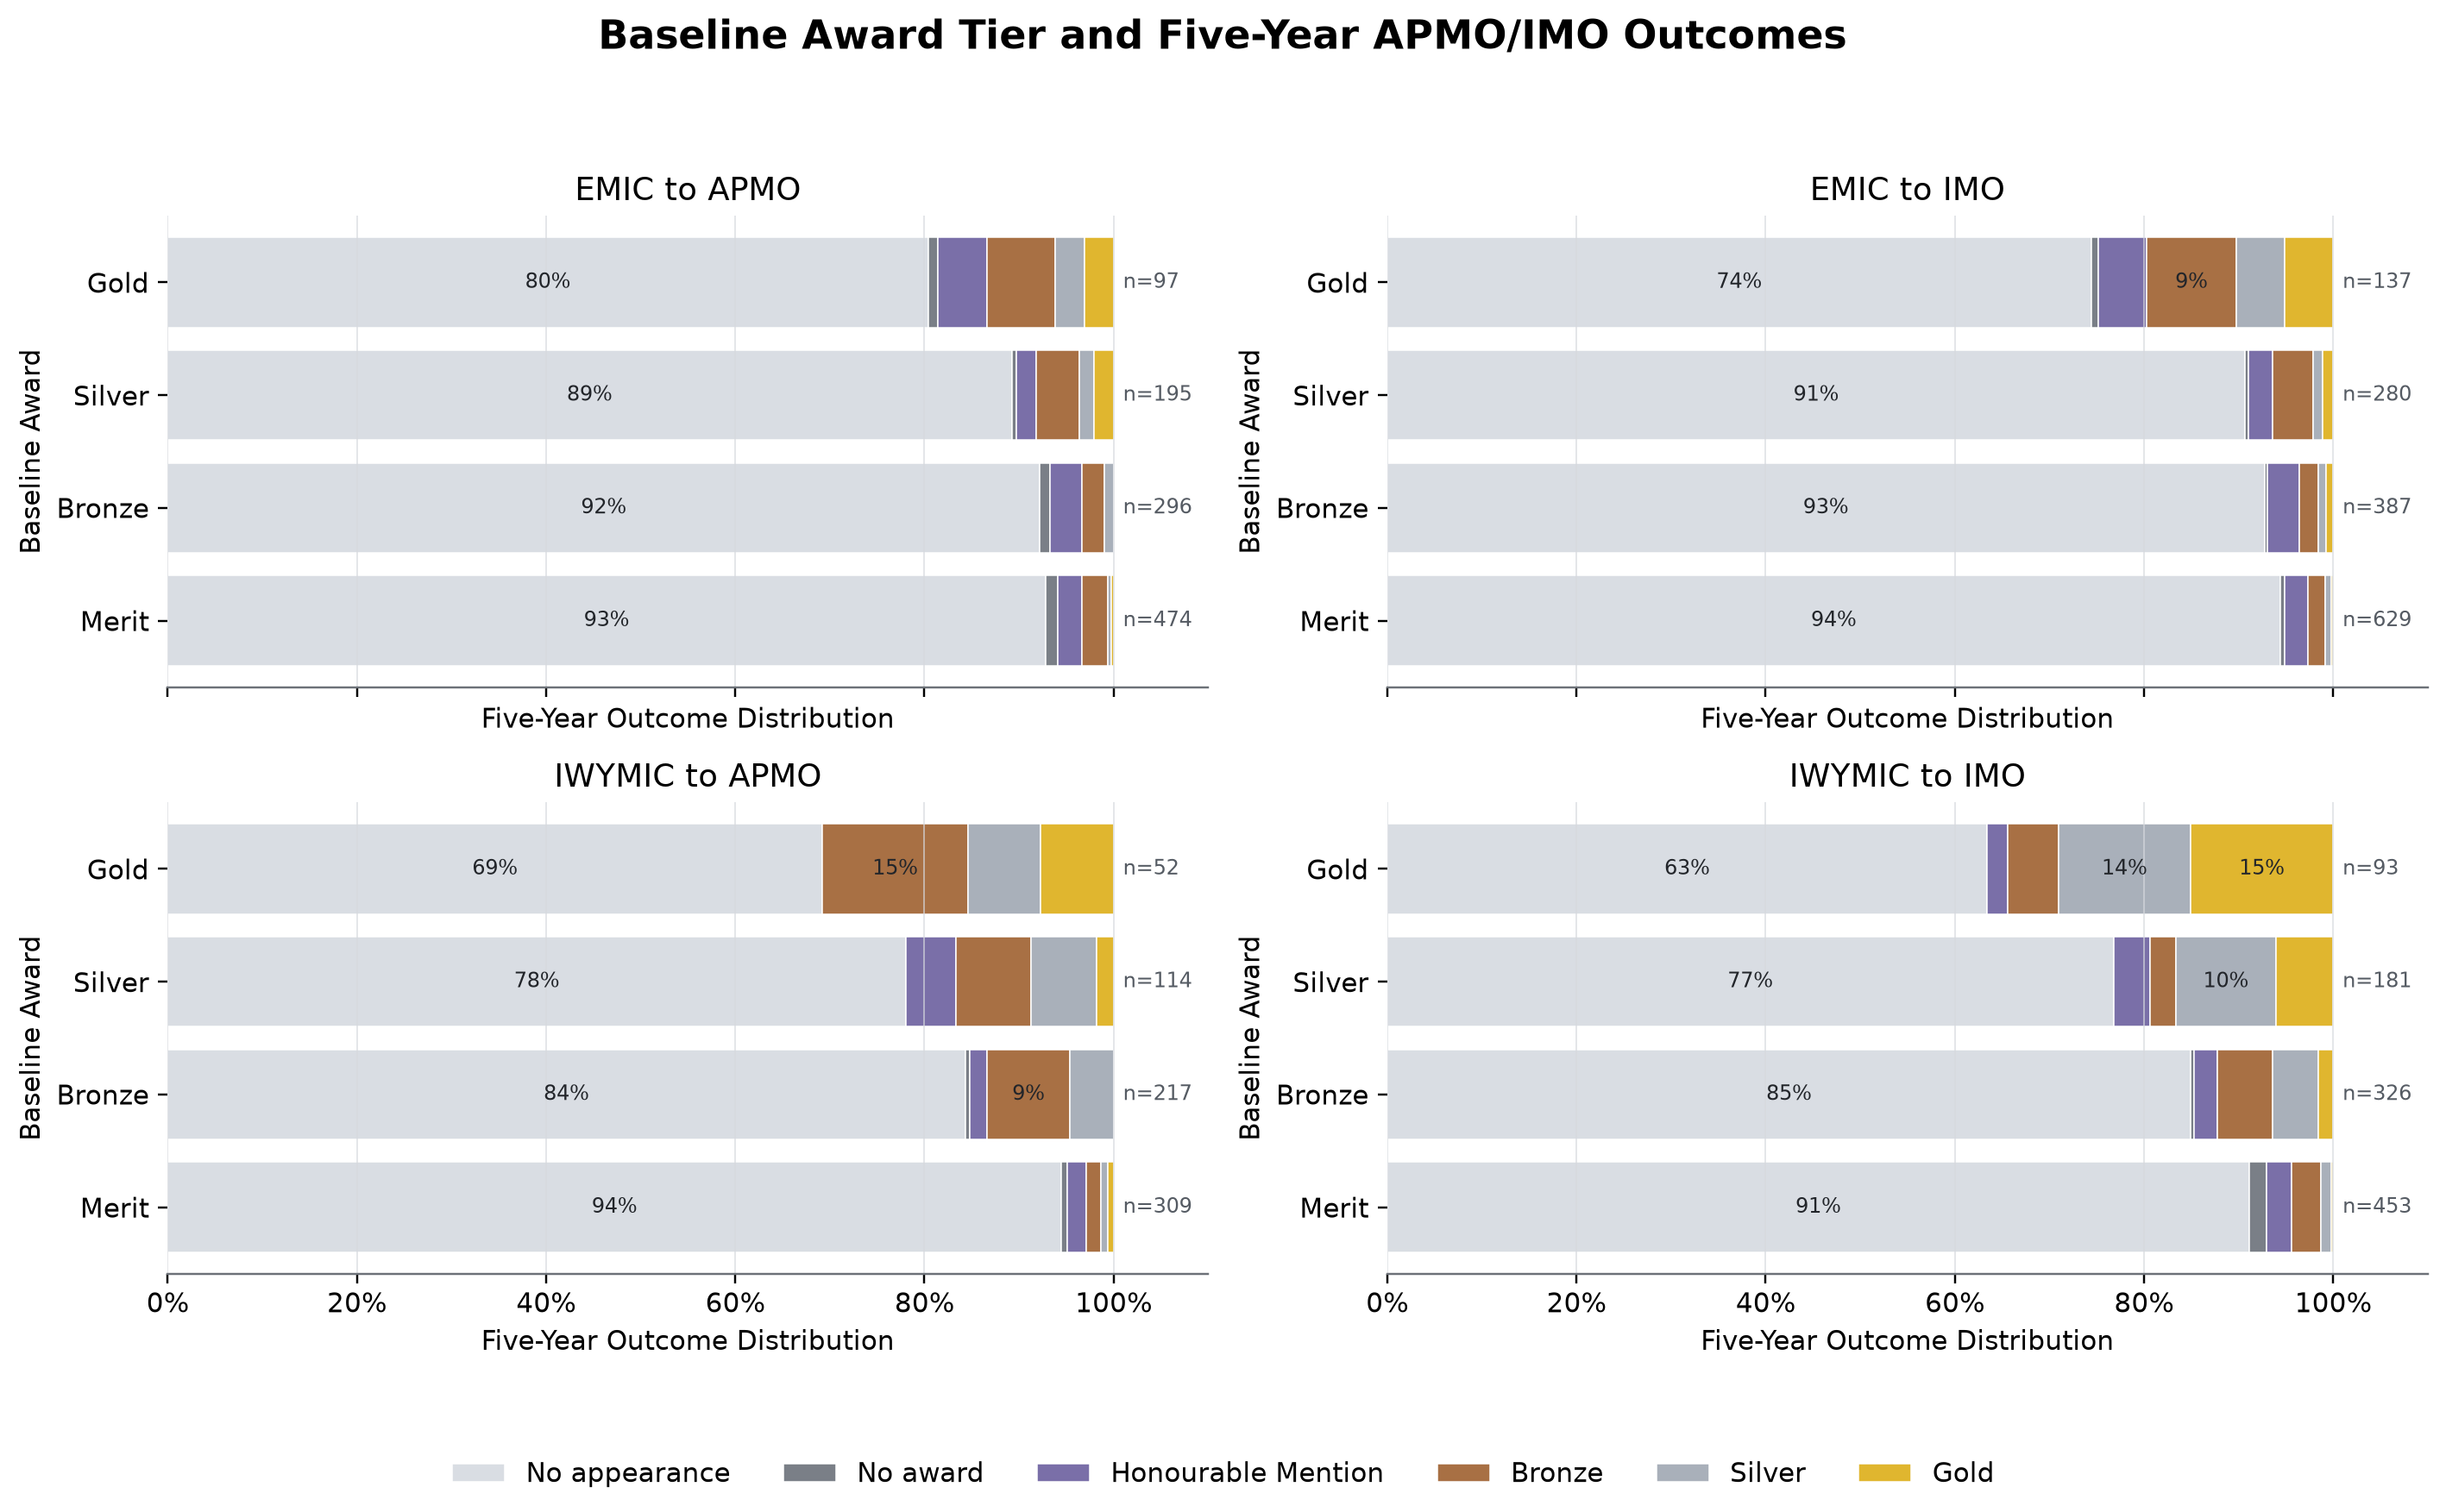
\includegraphics[width=\textwidth]{02 Outcome Transitions.png}
\caption{Distribution of later outcomes within five years, grouped by first observed stage and award tier.}
\end{figure}

The largest separation appears among IWYMIC recipients. IWYMIC Gold recipients have five-year award rates of 30.8\% for APMO and 36.6\% for IMO, compared with 4.9\% and 7.1\% for IWYMIC Merit recipients.

\section{Timing of Later Awards}

The time-to-event analysis retains incomplete recent cohorts by censoring each person at the end of 2026. It estimates the cumulative probability of receiving a later award among contestants whose outcome window begins within source coverage.

\begin{table}[H]
\centering
\caption{Five-Year Cumulative Award Incidence}
\small
\begin{tabular}{llrrrr}
\toprule
Destination & Baseline Band & Group & Estimate & Lower 95\% & Upper 95\% \\
\midrule
APMO & 25-50\% & 746 & 4.9\% & 3.3\% & 6.6\% \\
APMO & 50-75\% & 872 & 10.2\% & 8.1\% & 12.3\% \\
APMO & 75-100\% & 762 & 16.6\% & 13.8\% & 19.4\% \\
IMO & 25-50\% & 936 & 5.6\% & 4.0\% & 7.1\% \\
IMO & 50-75\% & 1,136 & 9.4\% & 7.6\% & 11.1\% \\
IMO & 75-100\% & 1,040 & 17.2\% & 14.8\% & 19.5\% \\
\bottomrule
\end{tabular}
\end{table}

\begin{figure}[H]
\centering
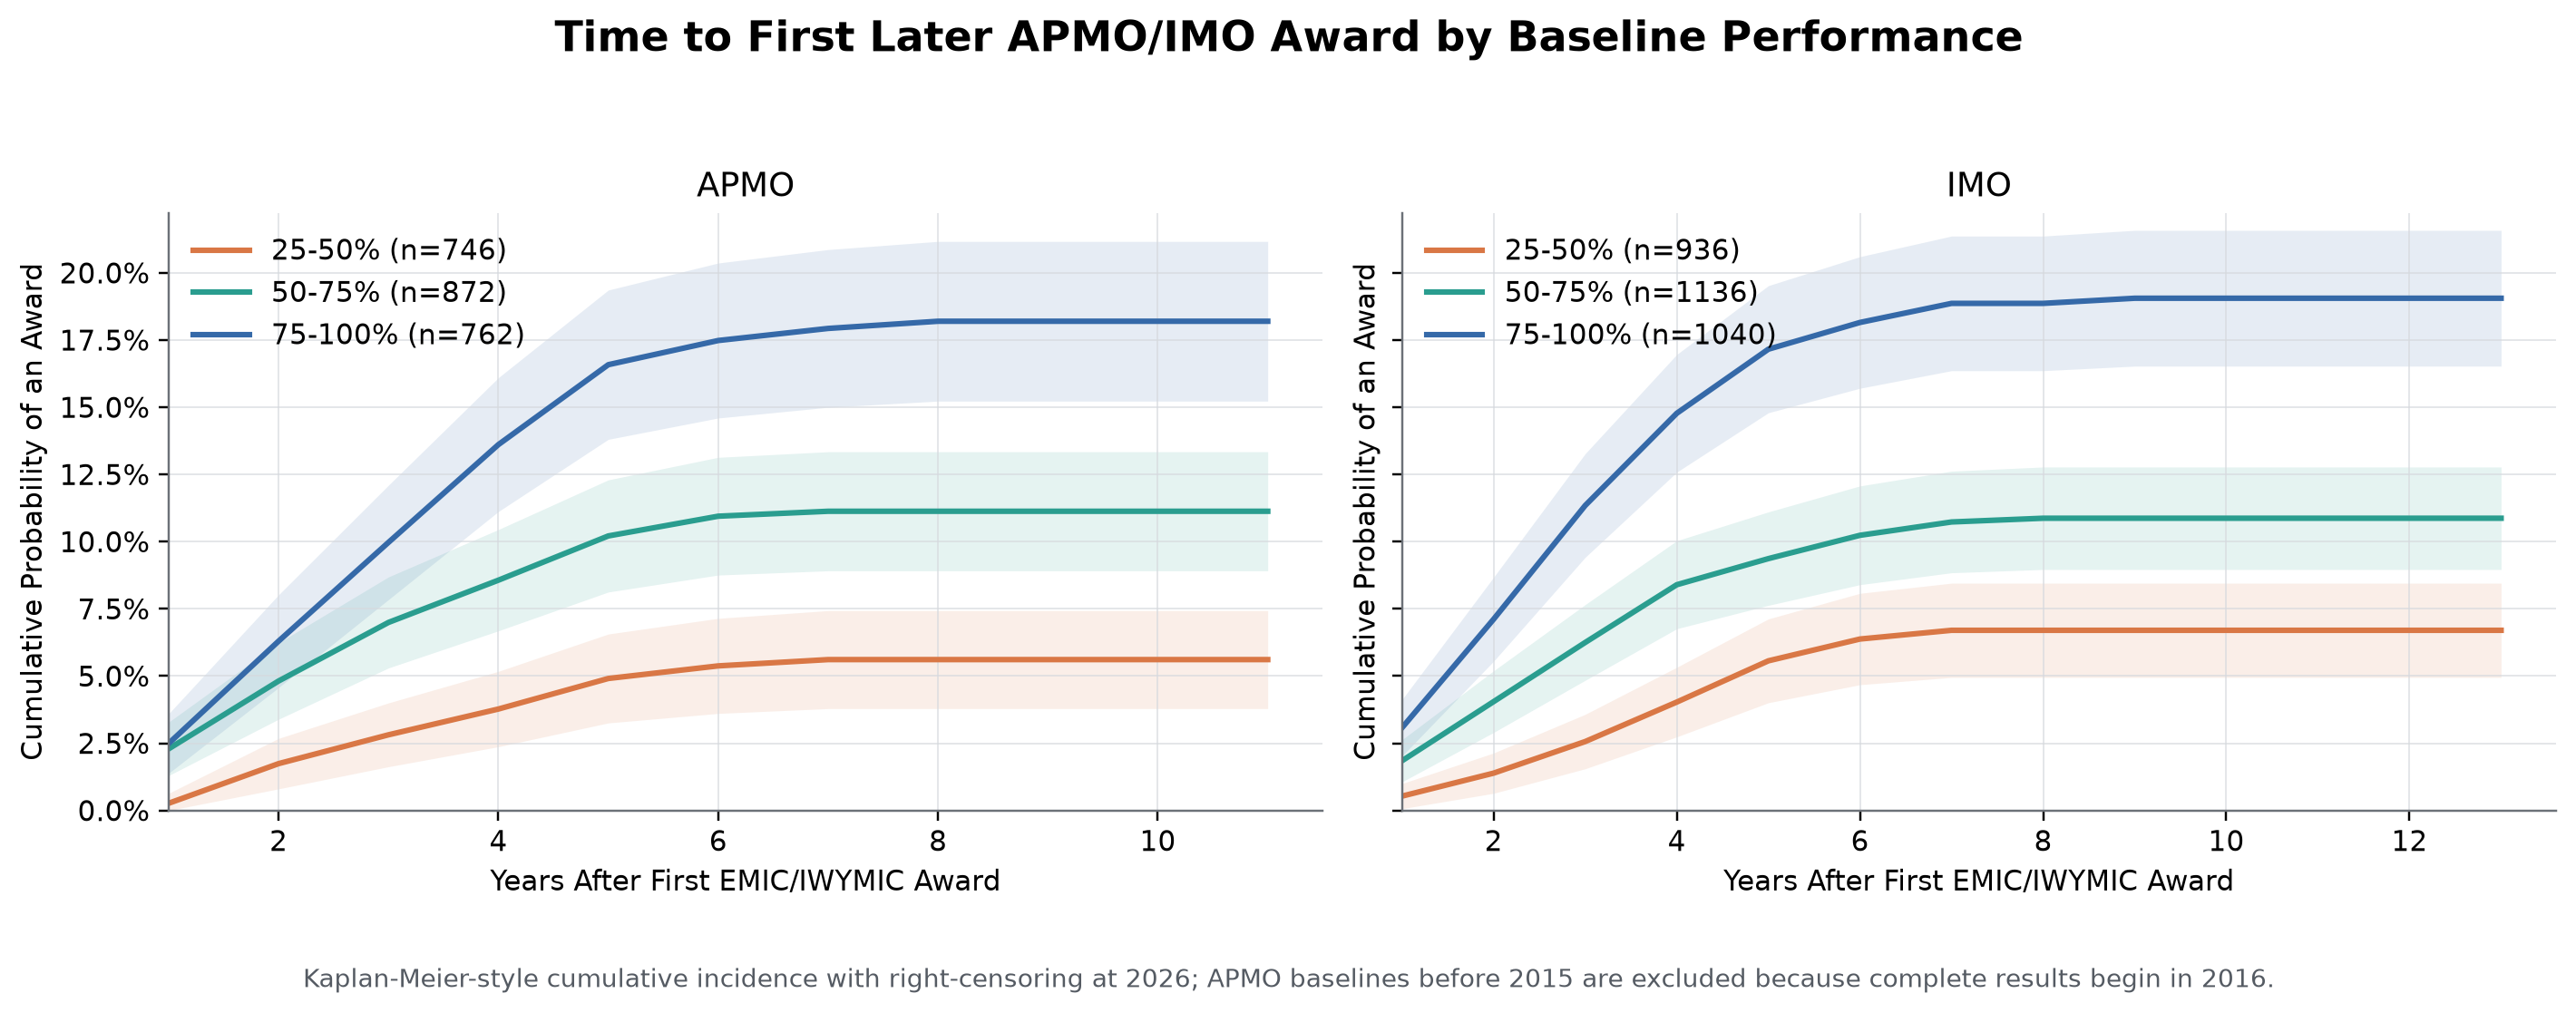
\includegraphics[width=\textwidth]{03 Cumulative Award Incidence.png}
\caption{Cumulative probability of a first later award with right-censoring at 2026.}
\end{figure}

Most separation develops within the first five to seven years after baseline. The curves then flatten because few new awards occur at longer lags and fewer contestants remain under observation.

\section{Country Context}

Country rates reflect both contestant performance and delegation systems. They should not be read as isolated measures of national program quality. Small samples can produce high point estimates with wide intervals.

\begin{table}[H]
\centering
\caption{Highest Five-Year Award Rates Among Countries With at Least 30 Eligible Contestants}
\small
\begin{tabular}{llrrrr}
\toprule
Destination & Country & Eligible & Awards & Rate & Wilson 95\% Interval \\
\midrule
APMO & Tajikistan & 44 & 23 & 52.3\% & 37.9\% to 66.2\% \\
APMO & Mexico & 47 & 22 & 46.8\% & 33.3\% to 60.8\% \\
APMO & Sri Lanka & 31 & 8 & 25.8\% & 13.7\% to 43.2\% \\
APMO & Kazakhstan & 46 & 8 & 17.4\% & 9.1\% to 30.7\% \\
APMO & Malaysia & 43 & 7 & 16.3\% & 8.1\% to 30.0\% \\
IMO & Uzbekistan & 33 & 16 & 48.5\% & 32.5\% to 64.8\% \\
IMO & Sri Lanka & 51 & 20 & 39.2\% & 27.0\% to 52.9\% \\
IMO & Tajikistan & 44 & 17 & 38.6\% & 25.7\% to 53.4\% \\
IMO & Singapore & 34 & 13 & 38.2\% & 23.9\% to 55.0\% \\
IMO & Mexico & 59 & 19 & 32.2\% & 21.7\% to 44.9\% \\
\bottomrule
\end{tabular}
\end{table}

\begin{figure}[H]
\centering
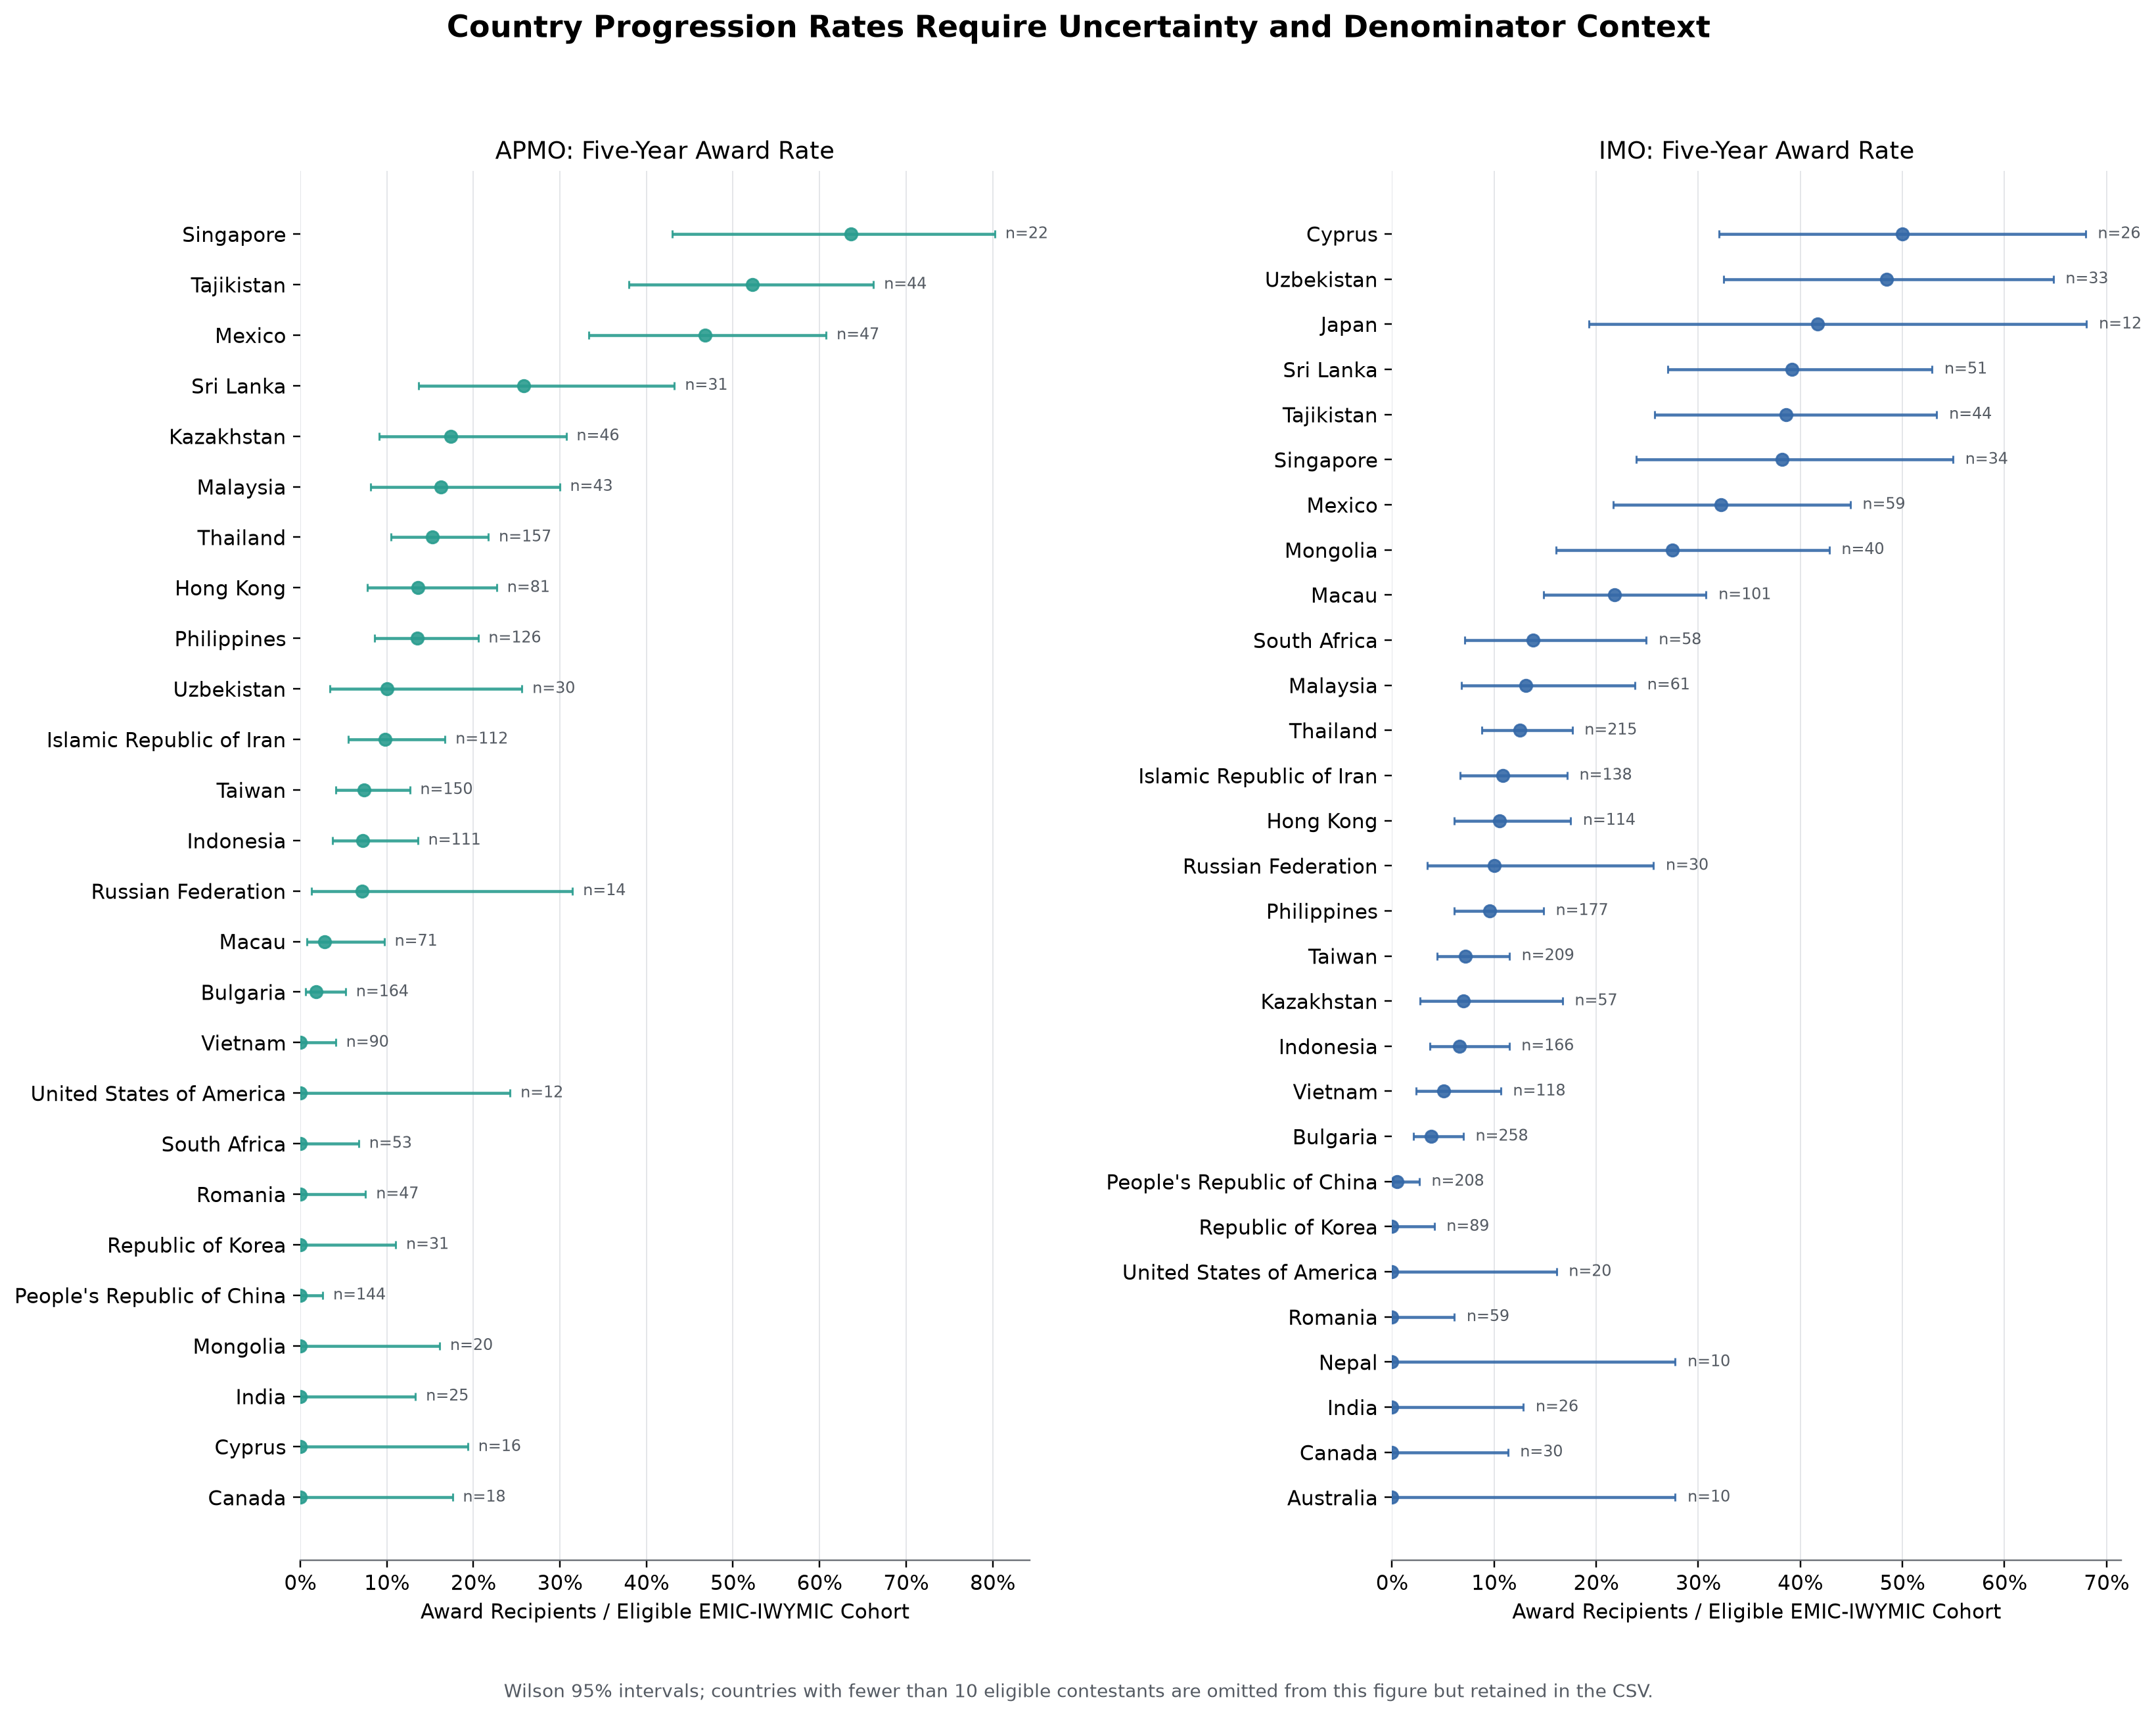
\includegraphics[width=0.88\textwidth]{04 Country Progression Rates.png}
\caption{Five-year country award rates. The figure shows countries with at least 10 eligible contestants; the table above applies a stricter threshold of 30.}
\end{figure}

The large country differences justify including country in the baseline model. They also show why raw cross-country comparisons can be misleading without denominator and uncertainty information.

\section{Out-of-Time Predictive Models}

Forward validation tests whether the model works on later cohorts. APMO predictions cover baseline years 2018, 2019, and 2021. IMO predictions cover 2016, 2017, 2018, 2019, and 2021. No model is trained on its test year or any later year.

\begin{table}[H]
\centering
\caption{Out-of-Time Predictive Performance}
\scriptsize
\begin{tabular}{lllrrrrr}
\toprule
Destination & Outcome & Model & Predictions & Events & Avg. Precision & ROC AUC & Brier \\
\midrule
APMO & Award & Baseline & 879 & 82 & 0.278 & 0.767 & 0.076 \\
APMO & Award & Performance & 879 & 82 & 0.365 & 0.838 & 0.071 \\
APMO & Medal & Baseline & 879 & 59 & 0.221 & 0.767 & 0.058 \\
APMO & Medal & Performance & 879 & 59 & 0.322 & 0.848 & 0.054 \\
IMO & Award & Baseline & 1,411 & 131 & 0.276 & 0.763 & 0.076 \\
IMO & Award & Performance & 1,411 & 131 & 0.351 & 0.809 & 0.072 \\
IMO & Medal & Baseline & 1,411 & 91 & 0.153 & 0.712 & 0.058 \\
IMO & Medal & Performance & 1,411 & 91 & 0.233 & 0.797 & 0.055 \\
\bottomrule
\end{tabular}
\end{table}

\begin{table}[H]
\centering
\caption{Incremental Value of Adding Baseline Performance}
\scriptsize
\begin{tabular}{llrrrrr}
\toprule
Destination & Outcome & $\Delta$ Avg. Precision & 95\% Interval & $\Delta$ ROC AUC & Brier Improvement & 95\% Interval \\
\midrule
APMO & Award & 0.088 & 0.033 to 0.161 & 0.071 & 0.004 & 0.000 to 0.009 \\
APMO & Medal & 0.101 & 0.034 to 0.189 & 0.081 & 0.004 & 0.001 to 0.007 \\
IMO & Award & 0.075 & 0.018 to 0.145 & 0.046 & 0.004 & 0.000 to 0.009 \\
IMO & Medal & 0.080 & 0.032 to 0.144 & 0.085 & 0.003 & 0.000 to 0.005 \\
\bottomrule
\end{tabular}
\end{table}

Average precision improves by 0.088 for APMO awards, 0.101 for APMO medals, 0.075 for IMO awards, and 0.080 for IMO medals. Every average-precision interval is above zero. Brier scores improve at the point estimate for all outcomes, although the IMO medal interval slightly crosses zero.

\begin{figure}[H]
\centering
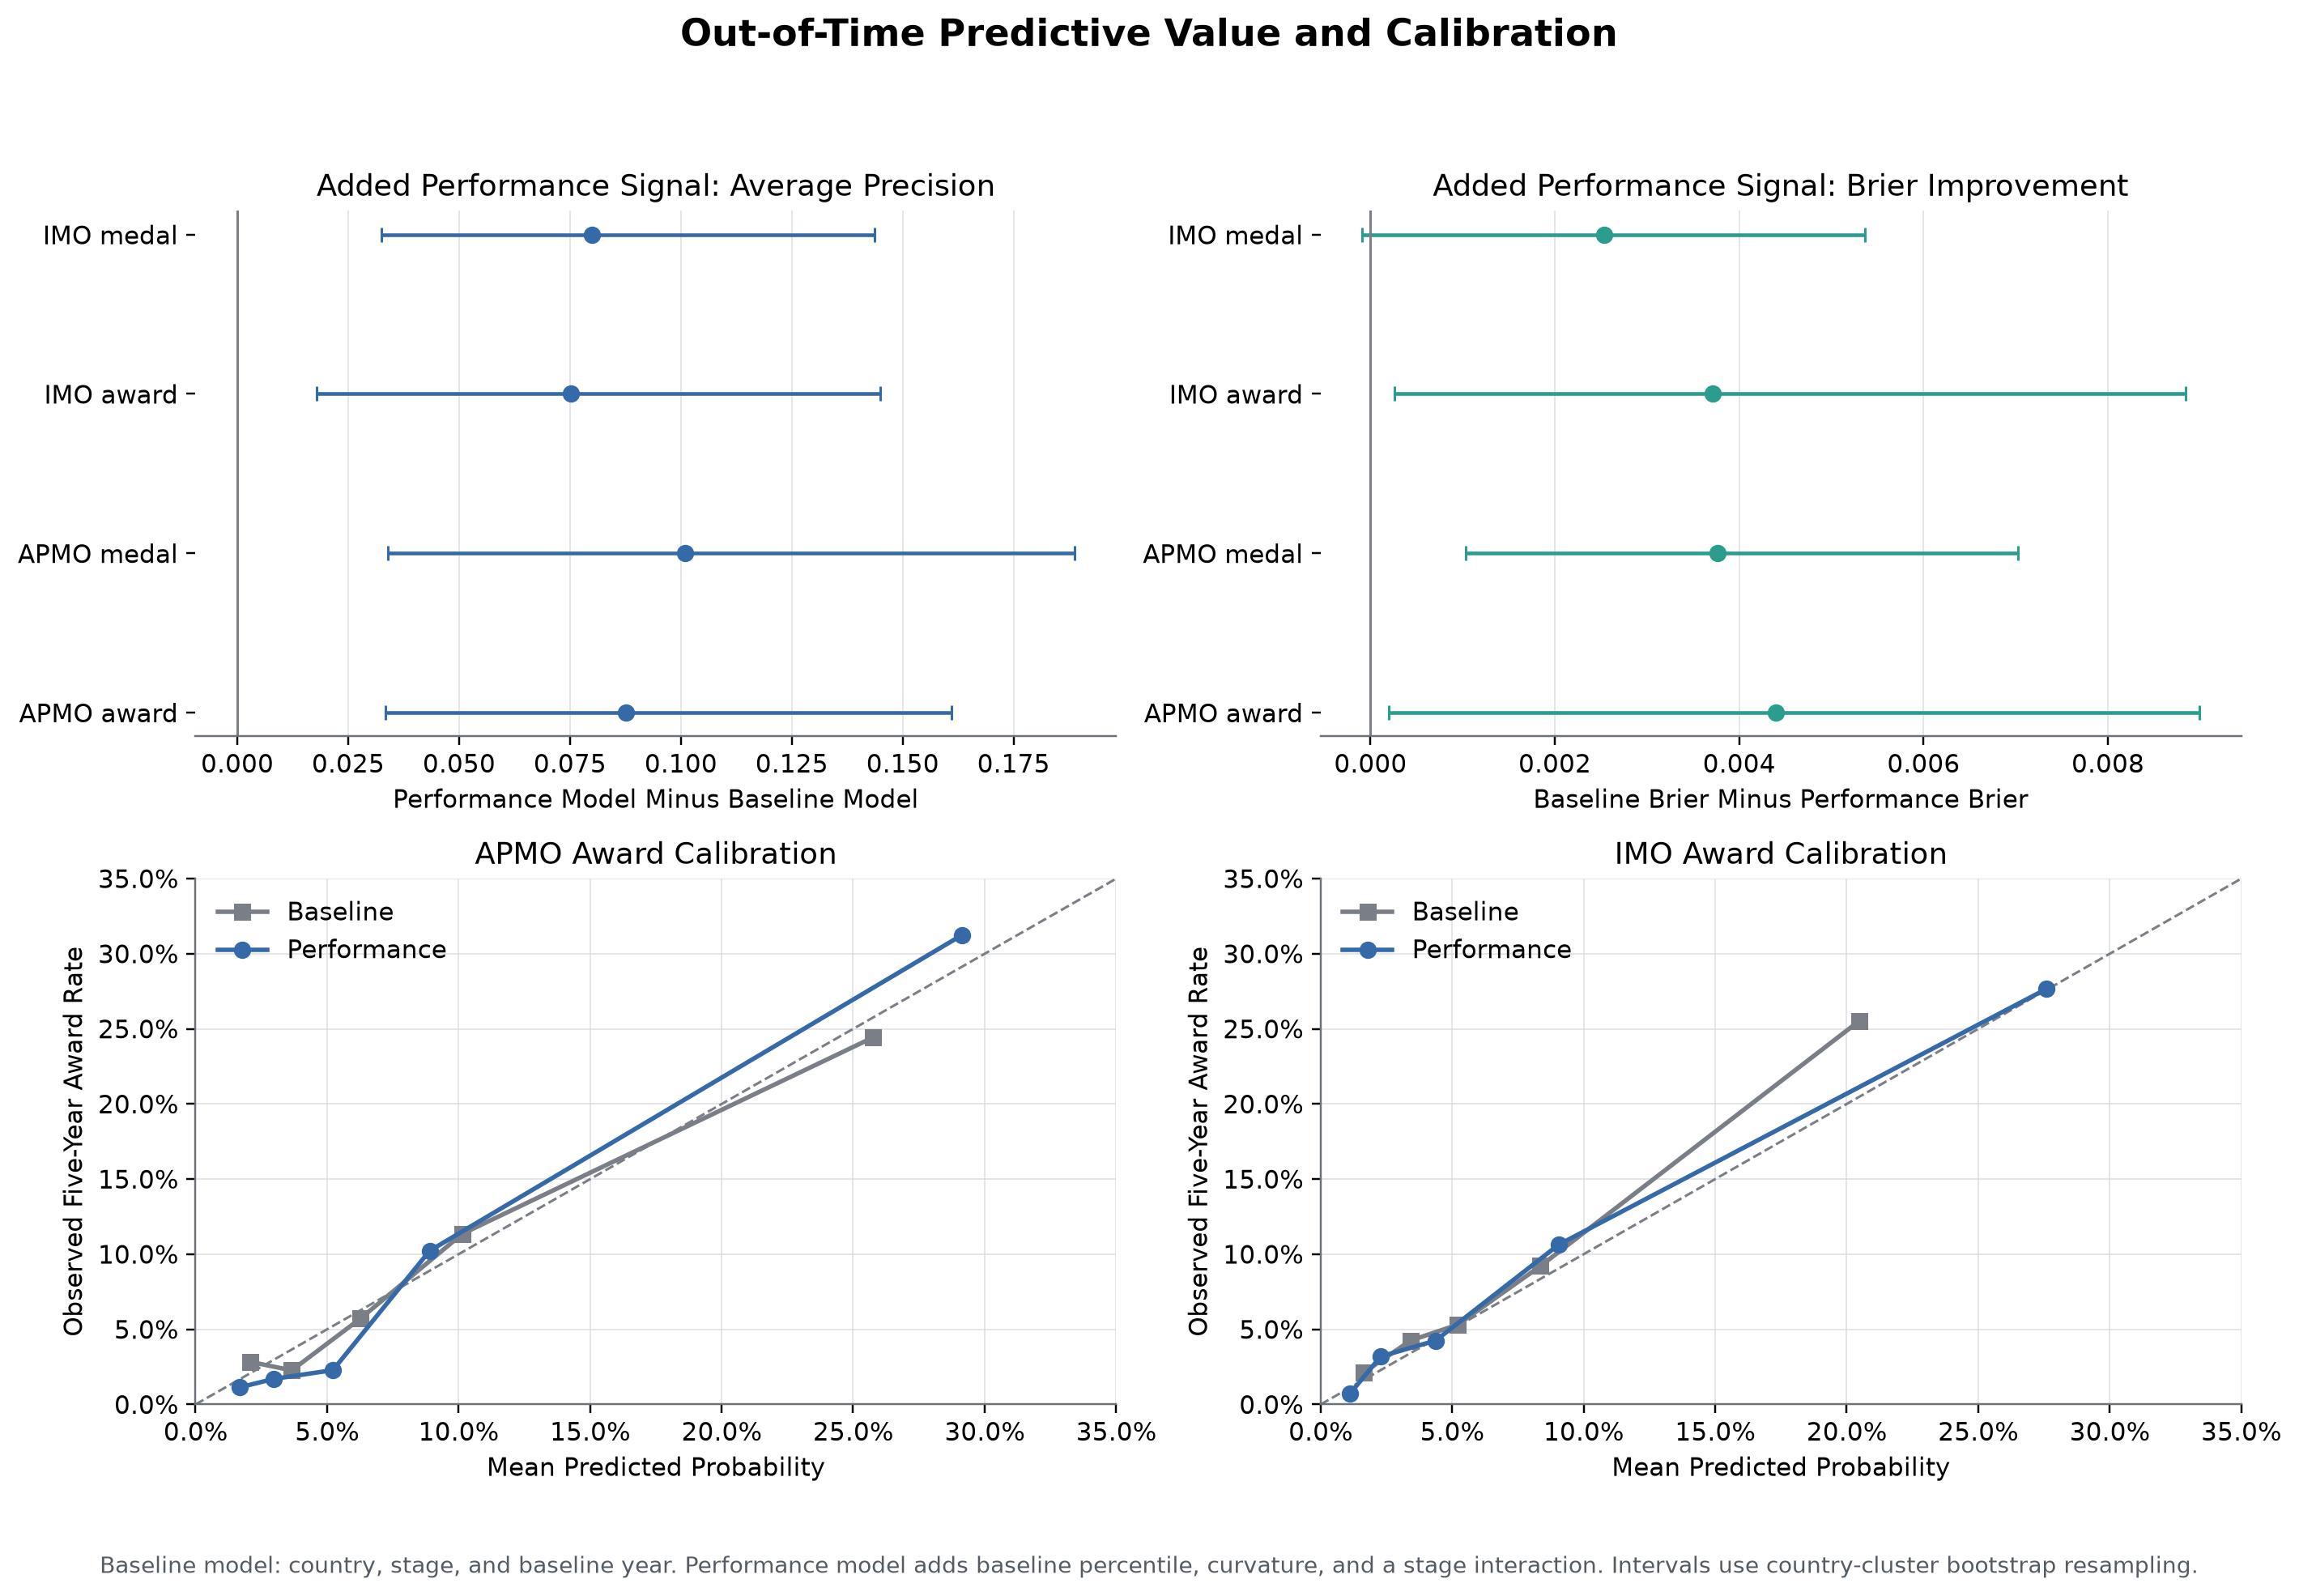
\includegraphics[width=\textwidth]{05 Model Comparison and Calibration.png}
\caption{Metric improvement and calibration for forward-year predictions. Positive improvement favors the performance model.}
\end{figure}

The performance model improves ranking and discrimination. Calibration remains broadly reasonable, but the highest-risk bins contain fewer events and therefore show more variation. The model is useful for group-level signal assessment. It is not suitable for deterministic predictions about individual students.

\section{Cohort Coverage}

Coverage determines which observations can support a fixed five-year outcome. Baselines from 2021 now have a complete five-year window because the higher-contest endpoint is 2026. Baselines from 2022 and 2023 remain incomplete and are excluded from fixed-window models.

\begin{figure}[H]
\centering
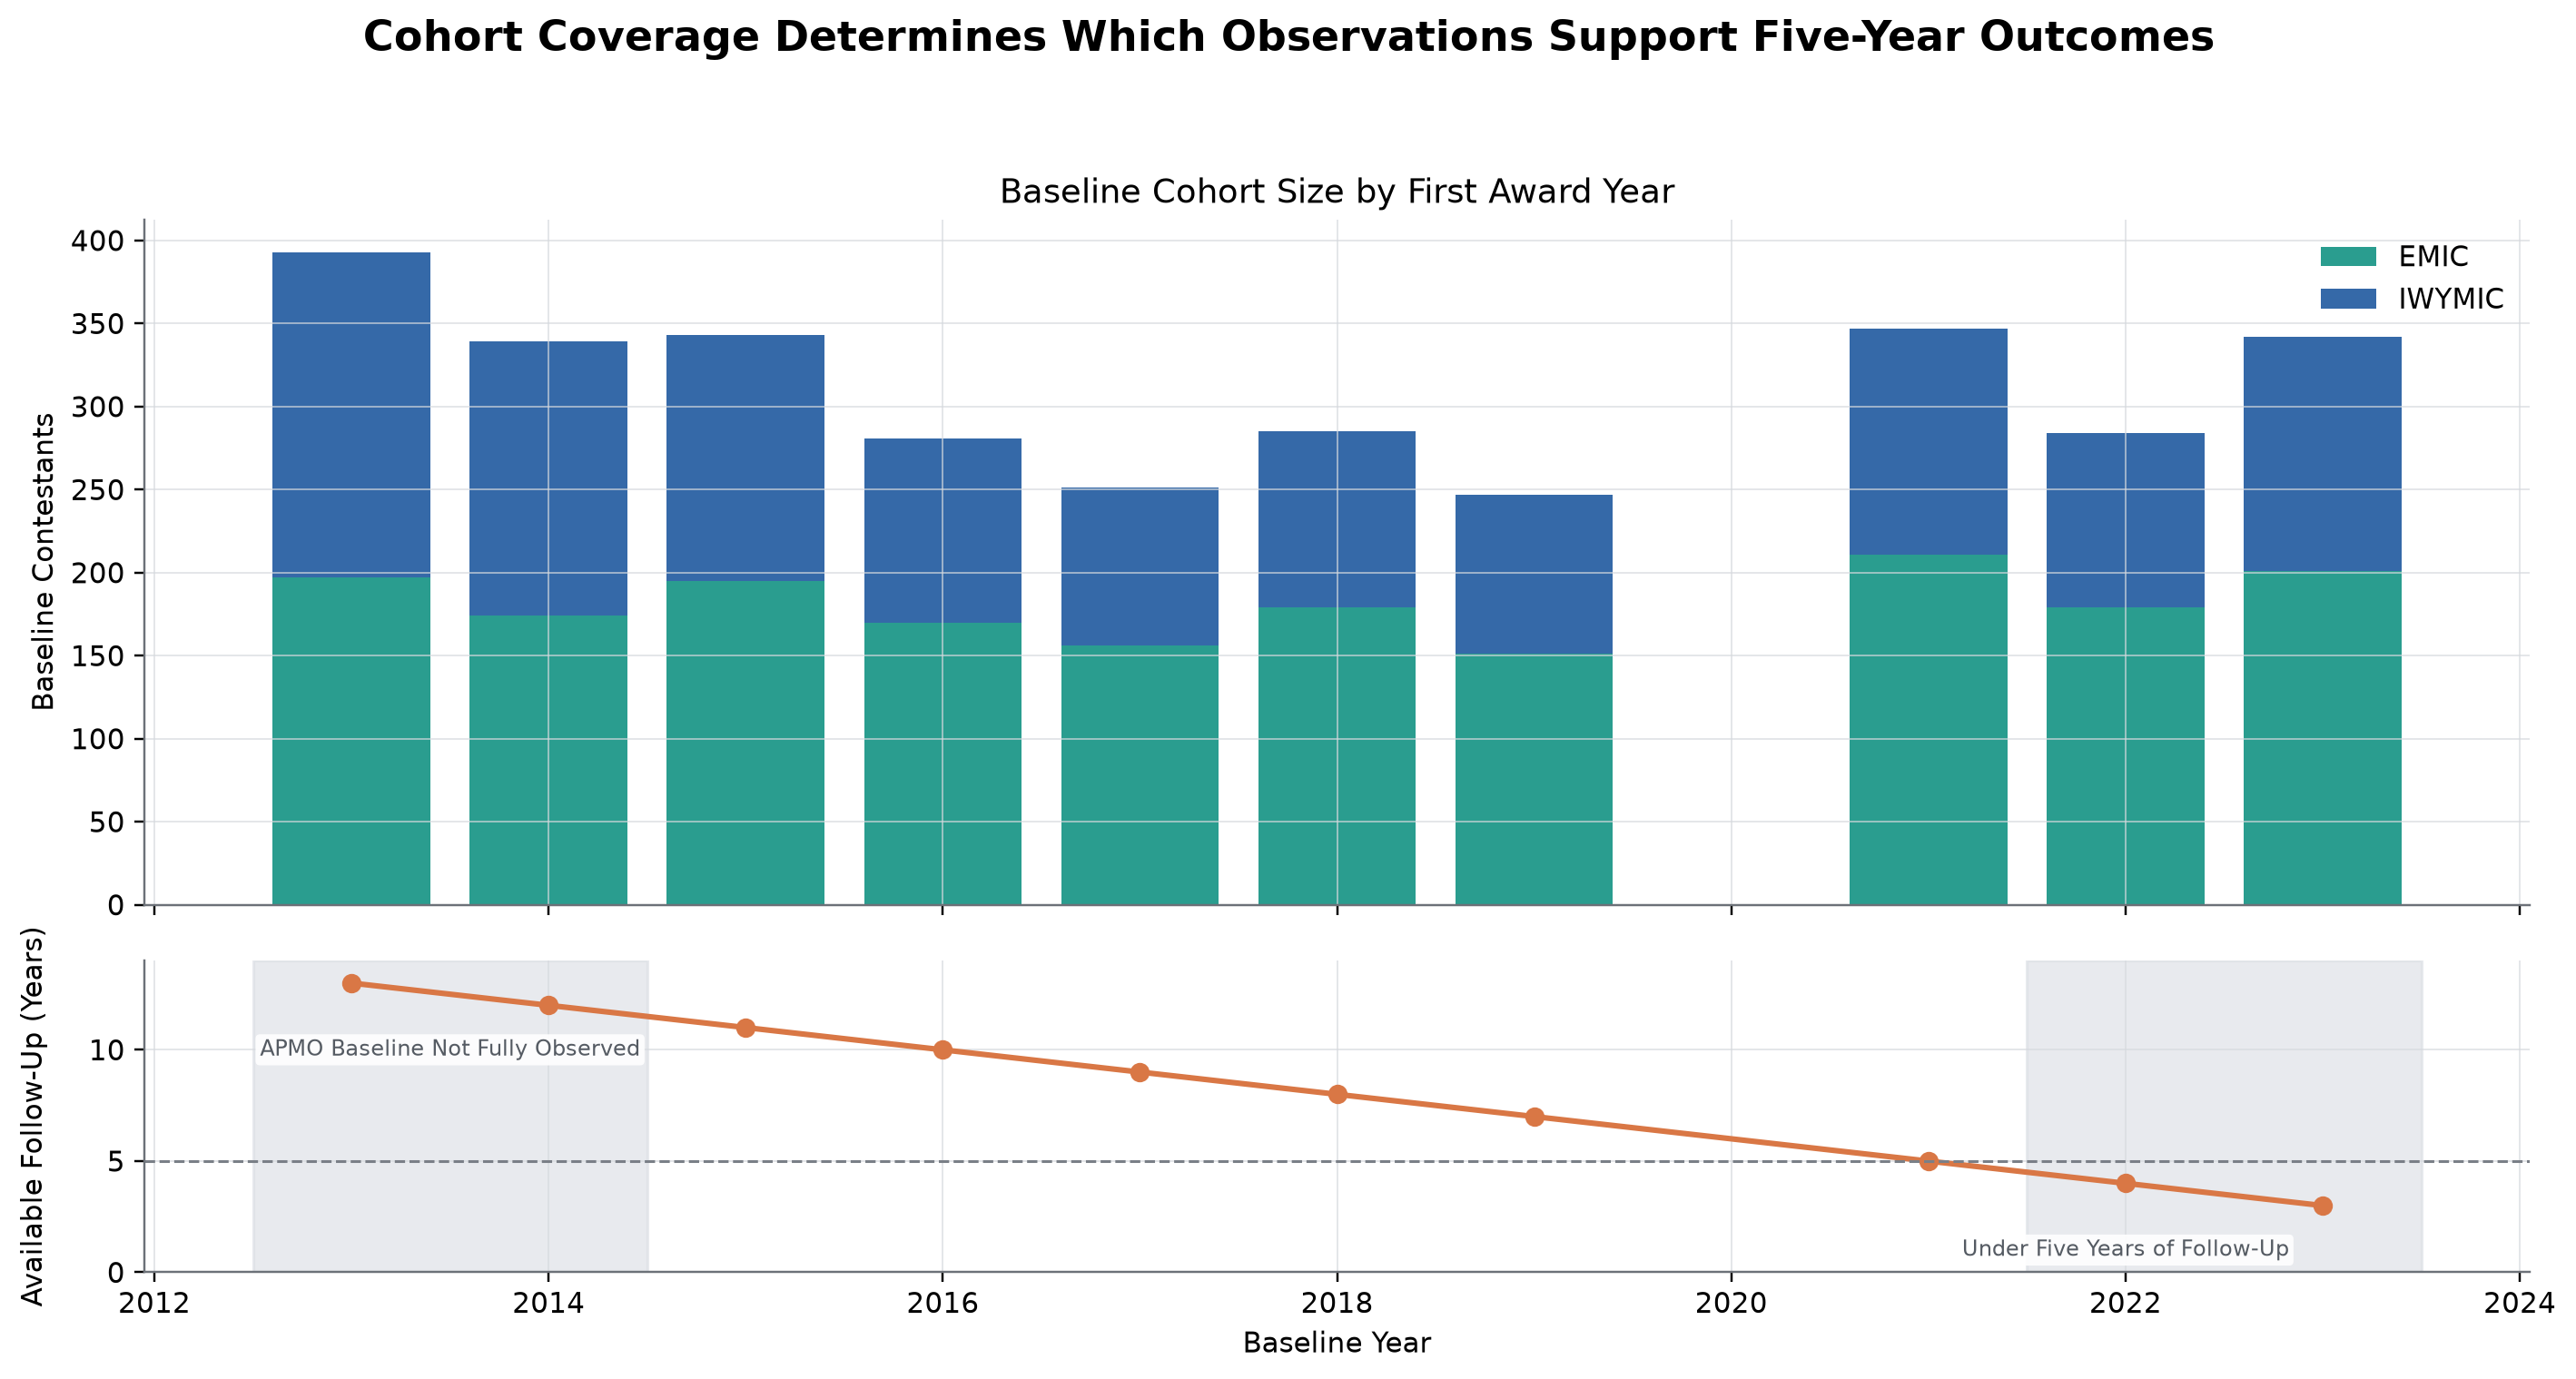
\includegraphics[width=\textwidth]{06 Cohort Coverage.png}
\caption{Baseline cohort sizes and available follow-up through 2026. Shading marks incomplete APMO source coverage and baselines with fewer than five follow-up years.}
\end{figure}

The 2026 update increases the five-year eligible samples to 1,754 for APMO and 2,486 for IMO. This is a substantive gain over the 2025 endpoint because an additional baseline cohort enters both model evaluation and descriptive fixed-window analyses.

\section{Answer to the Research Question}

\keyresult{\textbf{Conclusion.} Stronger EMIC/IWYMIC performance is a useful signal for later APMO and IMO success among named award recipients. The signal remains after adjustment for country, baseline year, and stage, and it improves prediction on later cohorts.}

The evidence does not show that EMIC or IWYMIC participation causes later success. Strong contestants may already have better preparation, training access, selection opportunities, or prior mathematical development. The appropriate interpretation is predictive association.

The evidence is strongest when several views agree:
\begin{itemize}
\item Percentile curves rise with baseline performance.
\item Medal-tier transitions show the same ordering.
\item Time-to-event estimates separate early and remain ordered.
\item Out-of-time models improve when performance is added.
\item Country adjustment reduces, but does not remove, the signal.
\end{itemize}

\section{Limitations}
\begin{itemize}
\item EMIC/IWYMIC result pages name award recipients only. Unnamed non-awardees cannot be followed, so the study does not compare all participants.
\item Country selection, training access, age, and prior preparation are not observed.
\item IWYMIC total-participant denominators are estimated. Medal-tier results provide an important sensitivity check.
\item APMO 2013 to 2015 lacks complete contestant-level score tables and is excluded from complete-window outcomes.
\item APMO 2026 is preliminary and may change when finalized.
\item Recent cohorts are right-censored. Fixed-window models intentionally exclude incomplete follow-up.
\item Identity matching is conservative. Ambiguous common names remain unmatched, which can slightly understate progression.
\end{itemize}

\section{Reproducibility and Output Inventory}

Run the statistical pipeline and report builder from the project root:

\begin{verbatim}
python "2 Processing Scripts/analyze_performance_signal.py"
python "2 Processing Scripts/build_statistical_analysis_report.py" --compile
\end{verbatim}

\begin{longtable}{p{0.35\textwidth}p{0.58\textwidth}}
\caption{Analysis Tables Used in This Report}\\
\toprule
File & Role \\
\midrule
\endfirsthead
\toprule
File & Role \\
\midrule
\endhead
Analysis Cohort.csv & One derived row per fixed identity \\
Descriptive Progression Summary.csv & Observed later outcomes by fixed performance band \\
Performance Band Summary.csv & Raw five-year quintile rates and Wilson intervals \\
Adjusted Signal Curves.csv & Country/year-adjusted probability curves \\
Outcome Transition Summary.csv & Baseline award tier to later result class \\
Survival Summary.csv & Right-censored cumulative award incidence \\
Country Progression Intervals.csv & Country rates and Wilson intervals \\
Cohort Coverage.csv & Baseline-year coverage and follow-up eligibility \\
Model Predictions.csv & Forward-year out-of-time probabilities \\
Model Results.csv & Predictive metrics by model and outcome \\
Model Comparison.csv & Incremental metrics with country bootstrap intervals \\
Calibration Summary.csv & Predicted and observed rates by probability bin \\
\bottomrule
\end{longtable}

The analysis code uses deterministic seeds for country-cluster bootstrap resampling. Generated tables, figures, the Markdown summary, this LaTeX source, the PDF, and source hashes are retained in \texttt{6 Statistical Analysis}.

\end{document}
